\chapter{As propriedades de translação e da transformada da integral}
\section{Propriedade de translação no eixo $s$}
Nessa seção vamos calcular a transformada inversa do deslocamento $F(s-a)$ sabendo a transformada inversa de $F(s)$. %O gráfico da figura \ref{fig_trans_1} mostra um exemplo de função com deslocamentos à direita e à esqueda.
\begin{teo}{\label{prop_trans_s}}(Propriedade da translação no eixo $s$) Se $F(s)$ é a transformada de Laplace de $f(t)$, então $e^{at}f(t)$ é a transformada inversa de $F(s-a)$, isto é
\begin{equation}
\mathcal{L}\left\{e^{at}f(t)\right\} =F(s-a),\qquad s>a
\end{equation}
ou
\begin{equation}{\label{eq_trans_s_inv}}
\mathcal{L}^{-1} \left\{F(s-a)\right\} =e^{at}f(t),\qquad s>a.
\end{equation} 
\end{teo}
\begin{proof}É direto da aplicação da definição da transformada de Laplace $F(s-a)$:
\begin{eqnarray*}
 F(s-a)&=&\int_0^\infty f(t)e^{-(s-a)t}dt\\
&=&\int_0^\infty f(t)e^{at}e^{-st}dt\\
&=&\mathcal{L}\left\{e^{at}f(t)\right\}
 \end{eqnarray*}
\end{proof}
Agora vamos calcular algumas transformadas de Laplace usando a propriedade \ref{prop_trans_s}.
\begin{ex}Para calcular a transformada de Laplace de $f(t)=te^{at}$, que é o item 8 da tabela \ref{tab_trans_Lap_1}, usamos o item 2 da mesma tabela,
\begin{equation}
\mathcal{L}\{t\}=\frac{1}{s^2}=F(s),
\end{equation}
e a propriedade de translação \ref{prop_trans_s} com $f(t)=t$:
\begin{equation}
\mathcal{L}\left\{e^{at}t\right\} =F(s-a)=\frac{1}{(s-a)^2},\qquad s>a
\end{equation}
\end{ex}
\begin{ex}Vamos provar o item 25 da tabela \ref{tab_trans_Lap_2},
\begin{equation}
\mathcal{L}\left\{ \frac{1}{4a^3}(\sen(at)\cosh(at)-\cos(at)\senh(at))\right\}=\frac{1}{s^4+4a^4},
\end{equation}
usando os itens 13 e 14 da tabela \ref{tab_trans_Lap_1}:
\begin{equation}
\mathcal{L}\left\{\frac{1}{a}\sen(at)\right\}=\frac{1}{s^2+a^2},
\end{equation}
e
\begin{equation}
\mathcal{L}\left\{\cos(at)\right\}=\frac{s}{s^2+a^2}.
\end{equation}
De fato,
\begin{small}
\begin{eqnarray*}
&&\mathcal{L}\left\{ \frac{1}{4a^3}(\sen(at)\cosh(at)-\cos(at)\senh(at))\right\}=\\
&&\qquad\qquad\quad=\mathcal{L}\left\{ \frac{1}{4a^3}\left(\sen(at)\frac{e^{at}+e^{-at}}{2}-\cos(at)\frac{e^{at}-e^{-at}}{2}\right)\right\}\\
&&\qquad\qquad\quad=\mathcal{L}\left\{ \frac{1}{8a^3}\left(e^{at}\left( \sen(at)-\cos(at)\right)+e^{-at}\left(\sen(at)+\cos(at)\right)\right)\right\}\\
&&\qquad\qquad\quad=\frac{1}{8a^3}\left[ \mathcal{L}\left\{ \left(e^{at}\left( \sen(at)-\cos(at)\right)\right\}+\mathcal{L}\left\{e^{-at}\left(\sen(at)+\cos(at)\right)\right)\right\}\right]\\
&&\qquad\qquad\quad=\frac{1}{8a^3}\left[\frac{a}{(s-a)^2+a^2}-\frac{s-a}{(s-a)^2+a^2}+\frac{a}{(s+a)^2+a^2}+\frac{s+a}{(s+a)^2+a^2}\right]\\
&&\qquad\qquad\quad=\frac{1}{8a^3}\left[\frac{8a^3}{\left((s-a)^2+a^2\right)\left((s+a)^2+a^2\right)}\right]\\
&&\qquad\qquad\quad=\frac{1}{s^4+4a^4}
\end{eqnarray*}
\end{small}
\end{ex}

\begin{ex}Vamos calcular a transformada de Laplace de $f(t)=e^{-t}\cosh(2t)$ usando a propriedade \ref{prop_trans_s} e a tabela \ref{tab_trans_Lap_1}. Primeiro observe o item 16 da tabela com $a=2$:
\begin{equation}
\mathcal{L}\{\cosh(2t)\}=\frac{s}{ s^2-4}=F(s).
\end{equation}
Agora use a propriedade da translação no eixo $s$
\begin{equation}
\mathcal{L}\left\{e^{-t}\cosh(2t)\right\} =F(s+1)=\frac{s+1}{ (s+1)^2-4},\qquad s>-1
\end{equation}
\end{ex}
\begin{ex}
 \item[a)] Agora vamos usar a propriedade \ref{prop_trans_s} e o item 15 da tabela \ref{tab_trans_Lap_1} para calcular a transformadas inversa de Laplace da função $F(s)=\frac{1}{s^2-2s-3}$. Primeiro escrevemos $F(s)$ numa forma conveniente:
\begin{equation}
F(s)=\frac{1}{s^2-2s-3}=\frac{1}{(s-1)^2-1-3}=\frac{1}{(s-1)^2-4}.
\end{equation}
Observe no item 16 da tabela que $\displaystyle\mathcal{L}\left\{\frac{1}{2}\senh(2t)\right\}=\frac{1}{ s^2-4}=G(s)$ e, também, pela propriedade da translação no eixo $s$ dada na equação (\ref{eq_trans_s_inv})
\begin{equation}
\mathcal{L}^{-1}\{F(s)\}=\mathcal{L}^{-1}\{G(s-1)\}=\frac{1}{2}e^{t}\senh(2t).
\end{equation}
\end{ex}
\subsection*{Exercícios}
\begin{exer}Use a propriedade \ref{prop_trans_s} e as tabelas \ref{tab_trans_Lap_1} e \ref{tab_trans_Lap_2} para calcular as seguintes transformadas de Laplace
\begin{itemize}
 \item[a)] $\displaystyle \mathcal{L}\left\{\frac{1}{(n-1)!}t^{n-1}e^{at}\right\}$\qquad (usando o item 3 da tabela)
 \item[b)] $\displaystyle \mathcal{L}\left\{\frac{1}{w}\sen(wt)e^{at}\right\}$\qquad (usando o item 13 da tabela)
\end{itemize}
\end{exer}
\begin{exer}Use a propriedade \ref{prop_trans_s} e as tabelas \ref{tab_trans_Lap_1} e \ref{tab_trans_Lap_2} para calcular as seguintes transformadas de Laplace
\begin{itemize}
 \item[a)] $\displaystyle \mathcal{L}\left\{\senh(2t)\cos(t)\right\}$
 \item[b)] $\displaystyle \mathcal{L}\left\{(4+t^2)e^t\right\}$
\end{itemize}
\end{exer}
\begin{exer}Encontre $f(t)$ dado que $F(s)$ usando as tabelas e as propriedades
\begin{itemize}
 \item[a)] $F(s)=\frac{s}{(s+1)^2+1}$
\item[b)] $F(s)=\frac{s-1}{(s^2-2s+5)(s^2-2s+10)}$
\end{itemize}
\end{exer}
\begin{exer}Use a propriedade \ref{prop_trans_s} e propriedade \ref{prop_trans_t} para calcular a transformada inversa de Laplace
\begin{equation}
F(s)=\frac{e^{-2s}(s-1)}{s^2 -2s+5}.
\end{equation}
\end{exer}
\begin{exer}
Utilize a propriedade do deslocamento no eixo $s$ para encontrar a transformada de Laplace de:
\begin{itemize}
  \item[a)] $t^2 e^{3t}$
  \item[b)] $e^{-2t} \sen {4t}$
  \item[c)] $e^{4t} \cosh (5t)$
  \item[d)] $e^{-2t} \left( 3 \cos(6t) - 5 \sen (6t) \right)$
  \end{itemize}
\end{exer}
\begin{resp}
\begin{itemize}
   \item[a)] $\displaystyle \frac{2}{(s-3)^3}$
  \item[b)] $\displaystyle \frac{4}{s^2 +4s +20}$
  \item[c)] $\displaystyle \frac{s-4}{s^2 - 8s - 9}$
  \item[d)] $\displaystyle \frac{3s -24}{s^2 +4s + 40}$
\end{itemize}
  \end{resp}
\section{Aplicação: Oscilador Harmônico}
Uma mola elástica com uma extremidade fixada prende um corpo de massa $m$ na outra extremidade (veja figura (\ref{massa-mola})). Conside que o corpo esteja sujeito a uma força de atrito proporcional a velocidade com constante de amortecimento $\gamma$ e a que mola obedeça a lei de Hooke com constante $k$.
\begin{figure}[!ht]
\begin{center}

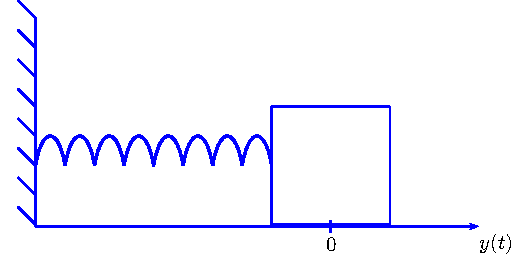
\includegraphics{cap_trans_int/pics/figura_1}\end{center}
\caption{\label{massa-mola}}
\end{figure} 
Seja $y(t)$ o deslocamento do corpo da sua posição de equilíbrio estático em função do tempo $t$. A equação do movimento é obtida a partir da segunda lei de Newton:
\begin{equation}
ma=\sum_i f_i,
\end{equation}
onde $a=y''(t)$ é a aceleração e $\sum_i \vec{f}_i$ representa a soma de todas as forças. No caso tratado aqui, existem apenas três forças, a saber:
\begin{itemize}
 \item[i)] a força da mola, que é proporcional ao descocamento (lei de Hooke), com constante de proporcionalidade $k$, $f_1=-k y(t)$,
 \item[ii)] a força de atrito, que é proporcional a velocidade, com constante de amortecimento $\gamma$, $f_2=-\gamma y'(t)$, e
 \item[iii)] a força externa, $f_3(t)=f(t)$
\end{itemize}
Logo,
\begin{equation}
my''(t)=f_1+f_2+f_3=-ky(t)-\gamma y'(t)+f(t),
\end{equation}
ou seja, a equação para o deslocamento $y(t)$ é dada por
\begin{equation}{\label{eq_massa_mola}}
my''(t)+\gamma y'(t)+ky(t)=f(t).
\end{equation}
O modelo fica completo quando impomos as condições iniciais $y(0)=y_0$ e $y'(0)=y_0'$. 
Agora, vamos usar o método da transformada de Laplace para resolver a equação. Aplicamos a transformada de Laplace na equação (\ref{eq_massa_mola}) e obtemos:
\begin{equation}
m\mathcal{L}\{y''(t)\}+\gamma \mathcal{L}\{y'(t)\}+k\mathcal{L}\{y(t)\}=\mathcal{L}\{f(t)\}.
\end{equation}
Aplicamos a propriedade \ref{prop_der} e obtemos
\begin{equation}
ms^2\mathcal{L}\{y(t)\}-msy(0)-my'(0)+\gamma s\mathcal{L}\{y(t)\}-\gamma y(0)+k\mathcal{L}\{y(t)\}=\mathcal{L}\{f(t)\}.
\end{equation}
Impomos as condições iniciais para obter a seguinte equação subsidiária:
\begin{equation}
ms^2Y(s)-msy_0-my_0'+\gamma sY(s)-\gamma y_0+kY(s)=F(s),
\end{equation}
onde $F(s)=\mathcal{L}\{f(t)\}$ e $Y(s)=\mathcal{L}\{y(t)\}$. Resolvemos a equação para $Y(s)$:
\begin{equation}
Y(s)=\frac{F(s)+msy_0+my_0'+\gamma y_0}{ms^2+\gamma s +k}.
\end{equation}
A solução do problema pode ser representado por $y(t)=\mathcal{L}^{-1}\{Y(s)\}$. 
O sistema massa mola pode ser classificado das seguintes formas:
\begin{itemize}
 \item[i)] Oscilador harmonico forçado: quando a força externa não é nula.
 \item[ii)] Oscilador harmônico livre: quando não há força externa, ou seja, $f(t)=0$, o que implica em $F(s)=0$. Nesse caso
\begin{equation}
Y(s)=\frac{msy_0+my_0'+\gamma y_0}{ms^2+\gamma s +k}.
\end{equation}
\item[iii)] Oscilador harmônico subamortecido: quando $\gamma^2< 4mk$. No caso $F(s)=0$, temos:
\begin{equation}
Y(s)=\frac{msy_0+my_0'+\gamma y_0}{ms^2+\gamma s +k}=\frac{msy_0+my_0'+\gamma y_0}{m\left(s+\frac{\gamma}{2m}\right)^2-\frac{\gamma^2}{4m} +k},
\end{equation}
onde $-\frac{\gamma^2}{4m} +k>0$. Olhando os itens 13 e 14 da tabela de transformada \ref{tab_trans_Lap_1} e combinando com a propriedade \ref{prop_trans_s}, concluímos que as soluções são são senos e cossenos multiplicados por exponenciais.
\item[iv)] Oscilador harmônico superamortecido: quando $\gamma^2> 4mk$. No caso $F(s)=0$, temos:
\begin{equation}
Y(s)=\frac{msy_0+my_0'+\gamma y_0}{ms^2+\gamma s +k}=\frac{msy_0+my_0'+\gamma y_0}{m\left(s+\frac{\gamma}{2m}\right)^2-\frac{\gamma^2}{4m} +k},
\end{equation}
onde $-\frac{\gamma^2}{4m} +k<0$. Olhando os itens 15 e 16 da tabela de transformada \ref{tab_trans_Lap_1} e combinando com a propriedade \ref{prop_trans_s}, concluímos que as soluções são são senos e cossenos hiperbólicos multiplicados por exponenciais, ou seja, somas de exponenciais puras (lembre-se que $\displaystyle 2\senh(at)=e^{at}-e^{-at}$ e $\displaystyle2\cosh(at)=e^{at}+e^{-at}$).
\item[v)] Oscilador harmônico criticamente amortecido: quando $\gamma^2= 4mk$. No caso $F(s)=0$, temos:
\begin{equation}
Y(s)=\frac{msy_0+my_0'+\gamma y_0}{ms^2+\gamma s +k}=\frac{msy_0+my_0'+\gamma y_0}{m\left(s+\frac{\gamma}{2m}\right)^2},
\end{equation}
Olhando para o item 3 da tabela de transformada \ref{tab_trans_Lap_1} e combinando com a propriedade \ref{prop_trans_s}, concluímos que as soluções são polinômios multiplicados por exponenciais.
\item[vi)] Oscilador harmônico não amortecido: quando $\gamma= 0$. No caso $F(s)=0$, temos:
\begin{equation}
Y(s)=\frac{msy_0+my_0'}{ms^2 +k}=\frac{sy_0+y_0'}{s^2+\frac{k}{m}},
\end{equation}
Olhando os items 13 e 14 da tabela de transformada \ref{tab_trans_Lap_1} concluímos que as soluções são senos e cossenos puros.
\end{itemize}
Para ilustrar, tomemos um caso subamortecido, por exemplo, $\gamma=2$, $m=1$ e $k=5$, sujeitos às condições iniciais $y_0=1$ e $y_0'=-2$. A função $Y(s)$ toma a forma: 
\begin{equation}
Y(s)=\frac{s}{s^2+2 s +5}.
\end{equation}
A transformada inversa nos leva a solução do problema:
\begin{equation}
y(t)=\mathcal{L}^{-1}\left\{\frac{s}{s^2+2 s +5}\right\}.
\end{equation}
Para calcular a inversa olhamos os itens 13 e 14 da tabela \ref{tab_trans_Lap_1} e escrevemos $\frac{s}{s^2+2 s +5}$ numa forma conveniente
\begin{equation}
\frac{s}{s^2+2 s +5}=\frac{s}{(s+1)^2 +4}=\frac{s+1}{(s+1)^2 +4}-\frac{1}{(s+1)^2 +4}.
\end{equation}
Usamos a propriedade \ref{prop_lin} para concluir o resultado
\begin{eqnarray*}
y(t)&=&\mathcal{L}^{-1}\left\{\frac{s+1}{(s+1)^2 +2^2}\right\}-\frac{1}{2}\mathcal{L}^{-1}\left\{\frac{2}{(s+1)^2 +2^2}\right\}\\
&=&e^{-t}\cos(2t)-\frac{1}{2}e^{-t}\sen(2t).
\end{eqnarray*}
Para identificar a amplitude e a fase, escrevemos a expressão em termos de exponencial vezes cosseno:
\begin{equation}
e^{-t}\left(\cos(2t)-\frac{1}{2}\sen(2t)\right)=Ae^{-t}\cos(2t+\delta)=Ae^{-t}\left(\cos(2t)\cos(\delta)-\sen(2t)\sen(\delta)\right).
\end{equation}
Isso é verdade se
\begin{eqnarray*}
A\cos(\delta)&=&1\\
A\sen(\delta)&=&\frac{1}{2}
\end{eqnarray*}
ou seja,
\begin{equation}
A=\sqrt{1+\frac{1}{4}}=\frac{\sqrt{5}}{2}
\end{equation}
e $\delta$ é uma fase no primeiro quadrante onde
\begin{equation}
\cos(\delta)=\frac{2}{\sqrt{5}}=\frac{2\sqrt{5}}{5},
\end{equation}
o que implica em $\delta\approx 0,463648\ \hbox{rad} \approx 26,57^0$. Portanto,
\begin{equation}
y(t)=\frac{\sqrt{5}}{2}e^{-t}\cos(2t+0,463648).
\end{equation}
A figura \ref{fig_massa_mola} ilustra o gráfico de $y(t)$.
\begin{figure}[!ht]
\begin{center}

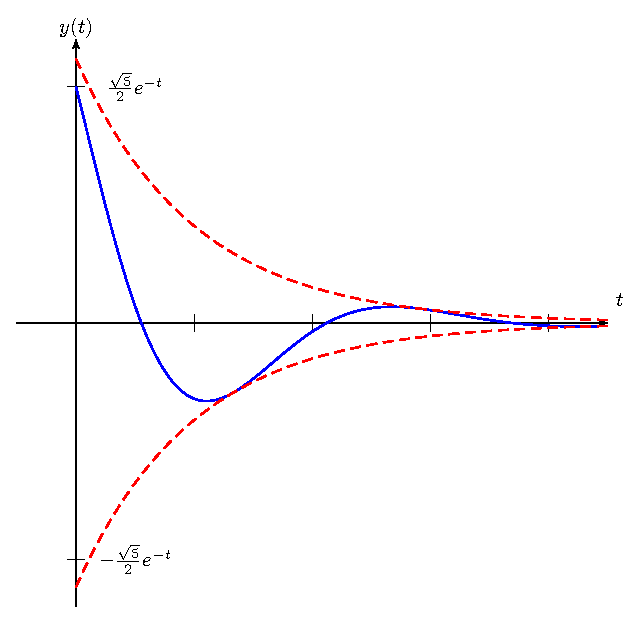
\includegraphics{cap_trans_int/pics/figura_2}\end{center}
{\caption{\label{fig_massa_mola}}}
\end{figure}

\subsection*{Exercícios}
\begin{exer}
Considere um oscilador harmônico modelado pelo problema de segunda ordem abaixo.

 \begin{eqnarray*}
my''(t)+\gamma y'(t)+ky(t)&=&0\\
y(0)&=&y_0\\
y'(0)&=&y_0'
\end{eqnarray*}
onde $m=3\!$ Kg, $\gamma=4\!$ Kg/s, $y_0=-1\!$ m, $y_0'=2\!$ m/s e $k$ é uma constante positiva. Encontre a faixa onde $k$ pode assumir valores para que o sistema fique superamortecido.
\end{exer}
\begin{resp}
 $0<k<\frac{4}{3}$.
\end{resp}
\begin{exer}Use a transformada de Laplace para resolver os seguintes problemas de valor inicial
\begin{itemize}
 \item[a)] $\displaystyle\left\{ \begin{array}{l}y''+5y'+6y=12e^t,\\ y(0)=1,\\y'(0)=-1 \end{array}\right.$
 \item[b)] $\displaystyle\left\{ \begin{array}{l}y''+5y'+6y=6u(t-3),\\ y(0)=1,\\y'(0)=-1 \end{array}\right.$
\end{itemize}
\end{exer}
\begin{resp}
\begin{itemize}
 \item[a)] $y(t)=-2e^{-2t}+e^{t}+2e^{-3t}$
 \item[b)] $y(t)=u(t)\left(2e^{-2t}-e^{-3t}\right)+u(t-3)\left(1-3e^{-2t+6}+2e^{-3t+9}\right)$
\end{itemize}
\end{resp}
\begin{exer}(Ressonância) Considere o oscilador harmônico não amortecido com termo forçante descrito pelo problema de valor inicial dado por:
\begin{equation}\left\{
\begin{array}{l}
 my''(t)+ky(t)=F(t)\\
 y(0)=0\\
 y'(0)=0
\end{array}
\right.,
\end{equation}
onde $F(t)=F_0\sen\left(\sqrt{\frac{k}{m}}t\right)$.
Use o método de transformada de Laplace para calcular a solução, observando que a frequência de oscilação natural do sistema coincide com a frequência do termo forçante.
\end{exer}
\begin{resp}
$\displaystyle y(t)=\frac{F_0}{2k}\left(\sen\left(\sqrt{\frac{k}{m}}t\right)-\sqrt{\frac{k}{m}}t\cos\left(\sqrt{\frac{k}{m}}t\right)\right)$
\end{resp}


\begin{exer}Considere o oscilador harmônico amortecido com termo forçante $F(t)=2(u(t-1)-u(t-2))$ descrito pelo problema de valor inicial
\begin{equation}\left\{
\begin{array}{l}
 y''(t)+3y'(t)+2y(t)=F(t)\\
 y(0)=0\\
 y'(0)=0
\end{array}
\right..
\end{equation}
Use o método de transformada de Laplace para calcular a solução.
\end{exer}
\begin{resp}
$\displaystyle y(t)=(1-2e^{-(t-1)}+e^{-2(t-1)})u(t-1)-(1-2e^{-(t-2)}+e^{-2(t-2)})u(t-2)$
\end{resp}
\begin{exer}
 Considere o seguinte problema de segunda ordem que modela um sistema massa-mola-amortecedor
\begin{eqnarray*}
 m y''(t) +\alpha y'(t) + \kappa y(t) &=& f(t)
 \end{eqnarray*}
Onde $f(t)$ é a força externa e a condições iniciais $y(0)$ e $y'(0)$ são nulas.
 Supondo $m=4$ e $\kappa=1$, responda às alternativas a seguir:
 \begin{itemize}
  \item [a)] Encontre o conjunto de valores $\alpha$ para que o sistema seja amortecido.
  \item [b)] Encontre o conjunto de valores $\alpha$ para que o sistema seja sub-amortecido.
  \item [c)] Encontre o conjunto de valores $\alpha$ para que o sistema seja criticamente amortecido.
  \item [d)] Encontre o conjunto de valores $\alpha$ para que o sistema seja superamortecido. 
  \item [e)] Encontre a resposta $y(t)$ do sistema criticamente amortecido quando $f(t)=\delta(t-1)$.
 \end{itemize}
\end{exer}
\begin{resp}
 \begin{itemize}
  \item [a)] $\alpha>0$
  \item [b)] $0<\alpha<4$
  \item [c)] $\alpha=4$
  \item [d)] $\alpha>4$
  \item [e)] $y(t)=\frac{1}{4} u(t-1) (t-1) e^{-\frac{t-1}{2}}$
 \end{itemize}
\end{resp}
\section{A função de Heaviside}
A {\bf função de Heaviside} ou {\bf função degrau unitário} é nula para argumento negativo e vale 1 para argumento positivo. Quando o argumento é zero a função não precisa estar definida (ou pode-se definir qualquer valor, dependendo do contexto, por exemplo $1/2$). Observe que esta é uma função contínua por partes:
\begin{equation}
 u(t)=\left\{ \begin{array}{ll} 0, &t<0\\1,&t>0. \end{array}\right.
\end{equation}
A função de Heaviside com descontinuidade em $t=a$ é da forma
\begin{equation}
 u(t-a)=\left\{ \begin{array}{ll} 0, &t<a\\1,&t>a. \end{array}\right.
\end{equation}
A figura \ref{fig_Heaviside} apresenta os gráficos de $u(t)$ e $u(t-a)$ para $a>0$.
\begin{figure}[!ht]
\begin{center}

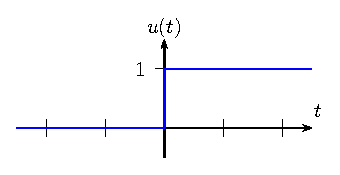
\includegraphics{cap_trans_int/pics/figura_3}
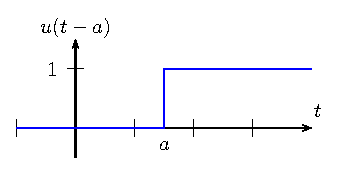
\includegraphics{cap_trans_int/pics/figura_4}\end{center}
\caption{\label{fig_Heaviside}}
\end{figure}
Observe que a representação gráfica em $t=a$ não está com o rigor matemático para funções, pois deveria estar esboçado bolinhas abertas indicando que em $t=a$ a função não está definida. Esse tipo de representação gráfico é usado no contexto de transformada de Laplace. Quando realmente for necessário definir um transição em $t=0$, toma-se uma aproximação linear e contínua para a função de Heaviside, chamada de {\bf função rampa}:
\begin{equation}
g_\epsilon(t)=\left\{\begin{array}{ll}0,& t<-\epsilon\\ \frac{1}{2\epsilon}t+\frac{1}{2},&-\epsilon\leq t \leq \epsilon\\1,&t>\epsilon, \end{array}\right.
\end{equation}
para $\epsilon<<1$. A figura \ref{fig_Heaviside_1} ilustra o gráfico de $g_\epsilon(t)$ para $\epsilon=1/2$.
\begin{figure}[!ht]
\begin{center}

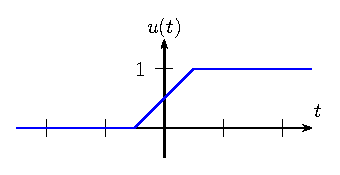
\includegraphics{cap_trans_int/pics/figura_5}\end{center}
\caption{\label{fig_Heaviside_1}}
\end{figure}
A função de Heaviside é o limite de $g_\epsilon(t)$ se $t\neq 0$:
\begin{equation}
\lim_{\epsilon\to 0}g_\epsilon(t) =u(t),\qquad t\neq 0.
\end{equation}
Uma função importante em aplicações é a {\bf função pulso}, definida por:
\begin{equation}
 f_p(t)=\left\{ \begin{array}{ll} 0, &t<a\\1,&a<t<b\\0,&t>b., \end{array}\right.
\end{equation}
com $a<b$
A figura \ref{fig_Heaviside_2} apresenta uma representação gráfica para a função pulso.
\begin{figure}[!ht]
\begin{center}

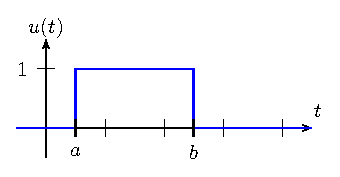
\includegraphics{cap_trans_int/pics/figura_6}\end{center}
\caption{\label{fig_Heaviside_2}}
\end{figure}
A função pulso normalmente é representada em termos da diferença de duas função de Heaviside:
\begin{equation}
f_p(t)=u(t-a)-u(t-b),\qquad a<b.
\end{equation}
A função pulso geralmente indica uma chave ``liga-desliga''. Por exemplo, o produto $f_p(t)f(t)$ significa que $f$ estava ``desligada'' para $t<a$, $f$ foi ``ligada'' em $t=a$ e ``desligada'' em $t=b$. Analogamente, o produto $u(t-a)f(t)$ indica que a função foi ligada em $t=a$. Observe o gráfico de $u(t-1)\sen(t)$ na figura \ref{fig_Heaviside_3}.
\begin{figure}[!ht]
\begin{center}

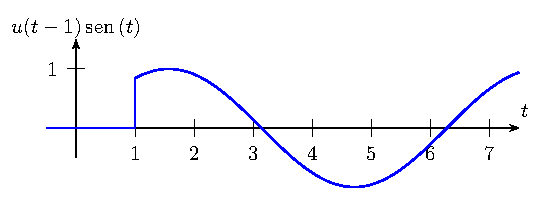
\includegraphics{cap_trans_int/pics/figura_7}\end{center}
\caption{\label{fig_Heaviside_3}Gráfico da função $u(t-1)\sen(t)$.}
\end{figure}
\begin{ex} Representar algebricamente em termos da função de Heaviside a função dada no gráfico da figura \ref{fig_Heaviside_4}.
\begin{figure}[!ht]
\begin{center}

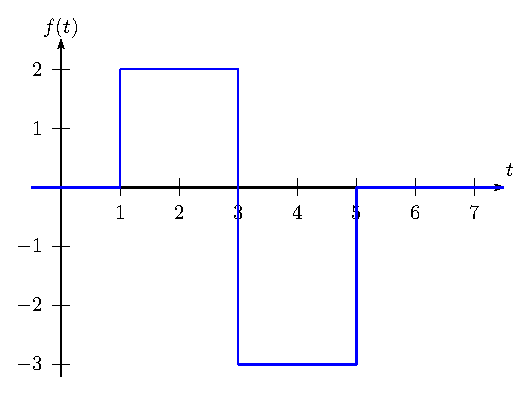
\includegraphics{cap_trans_int/pics/figura_8}\end{center}
\caption{\label{fig_Heaviside_4}}
\end{figure} 
Observe que podemos representar $f(t)$ da seguinte forma:
\begin{equation}
 f(t)=\left\{ \begin{array}{ll} 0, &t<1\\2,&1<t<3\\-3,& 3<t<5\\0,&t>5. \end{array}\right.
\end{equation}
Para representar em termos da função de Heaviside, olhe para o gráfico pensando em dois pulsos: $2(u(t-1)-u(t-3))$ e $-3(u(t-3)-u(t-5))$. A soma deles é a função desejada:
\begin{equation}
f(t)=2(u(t-1)-u(t-3))-3(u(t-3)-u(t-5)).
\end{equation}
\end{ex}

A transformada de Laplace da função de Heaviside é obtida direto da definição. Primeiro considere $a\geq 0$:
\begin{eqnarray}
\nonumber \mathcal{L}\{u(t-a)\}&=&\int_0^\infty u(t-a) e^{-st}dt\\
\nonumber &=&\int_a^\infty  e^{-st}dt\\
 &=&\left.  \frac{1}{-s}e^{-st}\right|_a^\infty=\frac{e^{-as}}{s}. {\label{Heaviside_trans}}
\end{eqnarray}
Se $a<0$, então
\begin{equation}
 \mathcal{L}\{u(t-a)\}=\mathcal{L}\{1\}=\frac{1}{s}.
\end{equation}

\subsection*{Exercícios}
\begin{exer}Esboce o gráfico da função $f(t)=(u(t)-u(t-2\pi))\sen(t)$.
\end{exer}
\begin{exer}Escreva uma expressão em termos da função de Heaviside para a função dada no gráfico \ref{fig_Heaviside_prob}.
 \begin{figure}[!ht]
\begin{center}

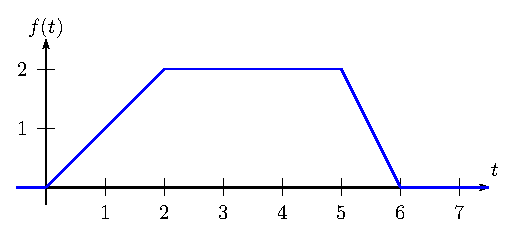
\includegraphics{cap_trans_int/pics/figura_9}\end{center}
\caption{\label{fig_Heaviside_prob}}
\end{figure} 
\end{exer}

\begin{exer}{\label{ex_Heaviside0}}Esboce o gráfico das seguintes funções:
\begin{itemize}
 \item [a)] $\displaystyle (t-\pi)u(t-\pi)$
 \item [b)] $\displaystyle t \ u(t-2)$
 \item [c)] $\displaystyle (\sen t) u(t-\pi)$
 \item [d)] $f(t)=u(t-1)+3u(t-3)-4u(t-5)$ 
 \item [e)] $f(t)=tu(t)+(t^2-t)u(t-1)+(6-t-t^2)u(t-2)+(t-6)u(t-6)$
 \item [f)] $f(t)=\left[u(t)+u(t-1)\right]^2$
 \item [g)] $f(t)=u(t-1)\left[1-u(t-2)\right] $
\end{itemize}
\end{exer}
\begin{resp}
 \begin{itemize}
 \item [a)] $\displaystyle (t-\pi)u(t-\pi)$
 \begin{center}

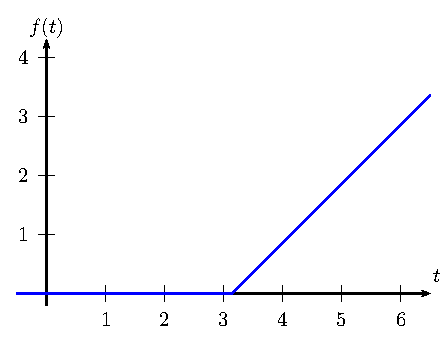
\includegraphics{cap_trans_int/pics/figura_13}\end{center}
 \item [b)] $\displaystyle t \ u(t-2)$
  \begin{center}

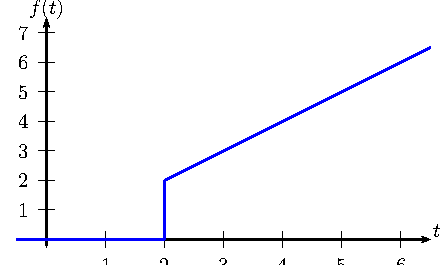
\includegraphics{cap_trans_int/pics/figura_14}\end{center}
 \item [c)] $\displaystyle (\sen t) u(t-\pi)$
 \begin{center}

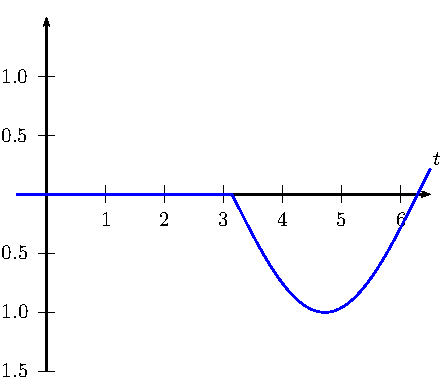
\includegraphics{cap_trans_int/pics/figura_15}\end{center}
\item[d)]$f(t)=u(t-1)+3u(t-3)-4u(t-5)$ 
\begin{center}

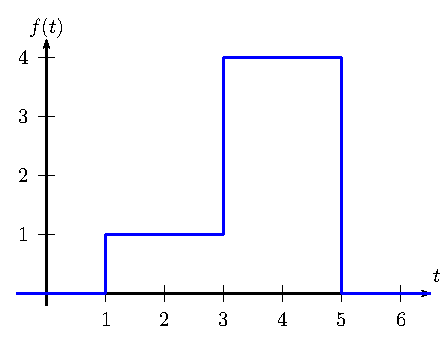
\includegraphics{cap_trans_int/pics/figura_16}\end{center}
\item[e)]$f(t)=tu(t)+(t^2-t)u(t-1)+(6-t-t^2)u(t-2)+(t-6)u(t-6)$
\begin{center}

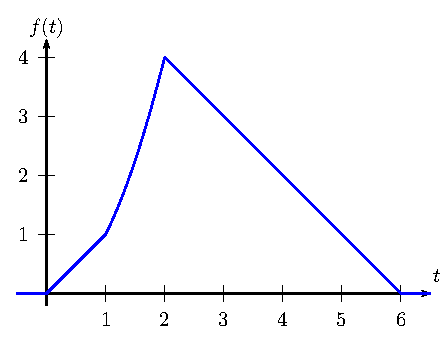
\includegraphics{cap_trans_int/pics/figura_17}\end{center}
\item[f)] $f(t)=\left[u(t)+u(t-1)\right]^2=u(t)+3u(t-1)$
\begin{center}

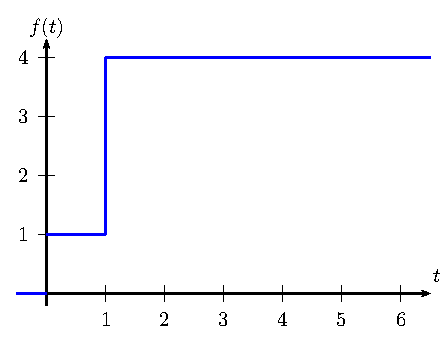
\includegraphics{cap_trans_int/pics/figura_18}\end{center}
 \item [g)] $f(t)=u(t-1)\left[1-u(t-2)\right]=u(t-1)-u(t-2) $
 \begin{center}

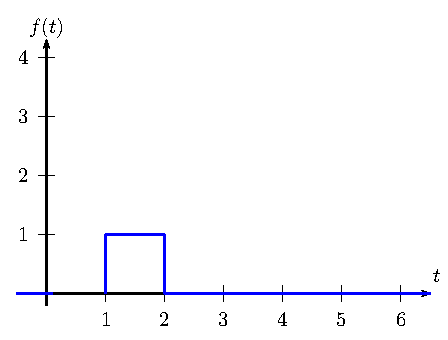
\includegraphics{cap_trans_int/pics/figura_19}\end{center}
\end{itemize}
\end{resp}


\begin{exer}{\label{ex_Heaviside1}}Escreva uma expressão para cada função em termos da função de Heaviside.
\begin{itemize}
\item[a)]~
\begin{center}

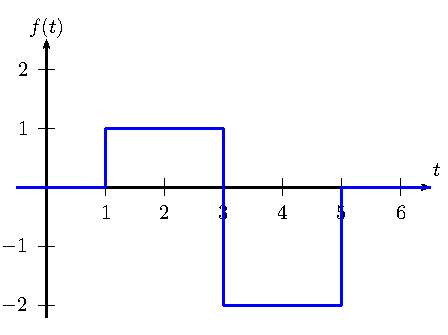
\includegraphics{cap_trans_int/pics/figura_20}\end{center}
\item[b)]~
\begin{center}

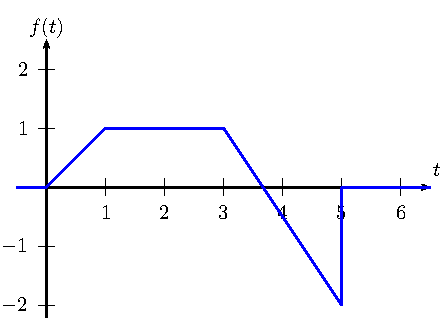
\includegraphics{cap_trans_int/pics/figura_21}\end{center}
\item[c)]~
\begin{center}

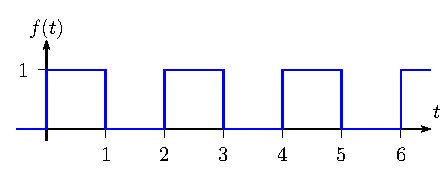
\includegraphics{cap_trans_int/pics/figura_22}\end{center}
\item[d)]~
\begin{center}

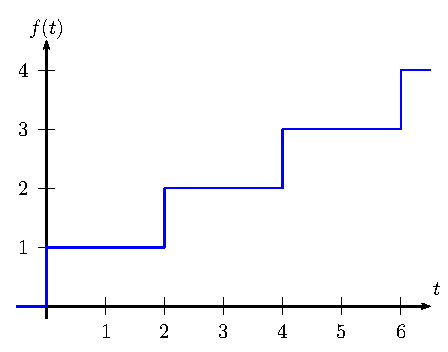
\includegraphics{cap_trans_int/pics/figura_23}\end{center}
\end{itemize}
\end{exer}
\begin{resp}
 \begin{itemize}
  \item[a)] $f(t)=u(t-1)-3u(t-3)+2u(t-5)$
    \item[b)] $f(t)=tu(t)+(1-t)u(t-1)+\left(-\frac{3}{2}t+\frac{9}{2}\right)u(t-3)+\left(\frac{3}{2}t-\frac{11}{2}\right)u(t-5)$
        \item[c)] $f(t)=\sum_{n=0}^\infty (-1)^n u(t-n)$
        \item[d)] $f(t)=\sum_{n=0}^\infty  u(t-2n)$ 
 \end{itemize}
\end{resp}

 \section{Propriedade do deslocamento no eixo $t$}
\begin{teo}{\label{prop_trans_t}}(Propriedade do deslocamento no eixo $t$) Se $F(s)$ é a transformada de $f(t)$, então $f(t-a)u(t-a)$ é a transformada inversa de $e^{-as}F(s)$, isto é
\begin{equation}
\mathcal{L}\left\{u(t-a)f(t-a)\right\} =e^{-as}F(s),\qquad a>0
\end{equation}
ou
\begin{equation}{\label{eq_trans_t_inv}}
\mathcal{L}^{-1} \left\{e^{-as}F(s)\right\} =u(t-a)f(t-a),\qquad a>0.
\end{equation} 
\end{teo}
\begin{proof}Aplicamos a definição da transformada de Laplace e obtemos:
\begin{eqnarray*}
\mathcal{L}\left\{u(t-a)f(t-a)\right\}&=&\int_0^\infty u(t-a)f(t-a)e^{-st}dt\\
&=&\int_0^a u(t-a)f(t-a)e^{-st}dt+\int_a^\infty u(t-a)f(t-a)e^{-st}dt\\
&=&\int_a^\infty f(t-a)e^{-st}dt,
\end{eqnarray*}
pois $u(t-a)$ é zero no intervalo $[0,a)$ e um no intervalo $(a,\infty)$. Depois usamos a mudança de variável $v=t-a$ na última integral:
\begin{equation*}
\int_a^\infty f(t-a)e^{-st}dt=\int_0^\infty f(v)e^{-s(v+a)}dv=e^{-as}\int_0^\infty f(v)e^{-sv}dv.
\end{equation*}
Logo,
\begin{equation}
\mathcal{L}\left\{u(t-a)f(t-a)\right\}=e^{-as}\mathcal{L}\left\{f(t)\right\}=e^{-as}F(s).
\end{equation}
\end{proof}
Observe que tomando $f(t)=1$ na propriedade \ref{prop_trans_t}, temos:
\begin{equation}{\label{Heaviside_trans_1}}
\mathcal{L}\left\{u(t-a)\right\} =\frac{e^{-as}}{s},\qquad a>0
\end{equation}
que coincide com a fórmula calculada na equação (\ref{Heaviside_trans}). Quando $a=0$ na equação (\ref{Heaviside_trans_1}), recaímos no item 1 da tabela \ref{tab_trans_Lap_1}.
\begin{ex} Aplicando diretamente a propriedade \ref{prop_trans_t} e usando que $\mathcal{L}\{t^2\}=\frac{2}{s^3}$, calculamos a transformada inversa de Laplace de $e^{-3s}\frac{2}{s^3}$:
\begin{equation}
\mathcal{L}^{-1}\left\{e^{-3s}\frac{2}{s^3}\right\}=u(t-3)(t-3)^2.
\end{equation}
\end{ex}
\begin{ex} Vamos calcular a transformada inversa de Laplace da função
\begin{equation}
F(s)=e^{-s}\frac{1}{(s+1)^2-1}.
\end{equation}
Primeiro calculamos a transformada de $\frac{1}{(s+1)^2-1}$ usando a propriedade \ref{prop_trans_s}
\begin{equation}
\mathcal{L}^{-1}\left\{\frac{1}{(s+1)^2-1}\right\}=e^{-t}\senh(t).
\end{equation}
Depois usamos a propriedade \ref{prop_trans_t} para concluir
\begin{equation}
\mathcal{L}^{-1}\left\{e^{-s}\frac{1}{(s+1)^2-1}\right\}=u(t-1)\mathcal{L}^{-1}\left\{\frac{1}{(s+1)^2-1}\right\}=u(t-1)e^{-(t-1)}\senh(t-1).
\end{equation}
\end{ex}

\subsection*{Exercícios}
\begin{exer}Use a propriedade \ref{prop_trans_t}, calcule a transformada inversa de Laplace e esboce um gráfico para cada item:
\begin{itemize}
\item[a)] $G(s)=e^{-2s}\frac{s}{s^2+4}$
\item[b)] $G(s)=e^{-s}\frac{1}{s^2}-3e^{-3s}\frac{1}{s^2}$
\end{itemize}
\end{exer}


\begin{exer} Calcule a transformada de Laplace para cada item do exercício \ref{ex_Heaviside0}.
\end{exer}
\begin{resp}
 \begin{itemize}
 \item [a)] $F(s)=\displaystyle \frac{e^{-\pi s}}{s^2}$
 \item [b)] $F(s)=\displaystyle e^{-2s}\bigg(\frac{1}{s^2}  + \frac{2}{s}\bigg)$
 \item [c)] $F(s)=\displaystyle - \frac{e^{-\pi s}}{s^2 +1}$
 \item [d)] $F(s)=\frac{1}{s}\left(e^{-s}+3e^{-3s}-4e^{-5s}\right)$
 \item [e)] $F(s)=\frac{1}{s^2}+\left(\frac{2}{s^3}+\frac{1}{s^2}\right)e^{-s}+\left(-\frac{2}{s^3}-\frac{5}{s^2}\right)e^{-2s}+\frac{1}{s^2}e^{-6s}$ 
 \item [f)]$F(s) = \frac{1+3e^{-s}}{s}$
 \item [g)] $F(s) = \frac{e^{-s}-e^{-2s}}{s}$ 
 \end{itemize}
\end{resp}
\begin{exer} Calcule a transformada de Laplace para cada item do exercício \ref{ex_Heaviside1}.
\end{exer}
\begin{resp}
 \begin{itemize}
  \item[a)] $F(s)=\frac{1}{s}\left(e^{-s}-3e^{-3s}+2e^{-5s}\right)$
    \item[b)] $F(s)=\frac{1}{s^2}\left(1-e^{-s}-\frac{3}{2}e^{-3s}+\frac{3}{2}e^{-5s}+2se^{-5s}\right)$
        \item[c)] $F(s)=\frac{1}{s(1+e^{-s})}$
        \item[d)] $F(s)=\frac{1}{s(1-e^{-2s})}$ 
 \end{itemize}
\end{resp}
\begin{exer} Use os itens c) e d) do exercício \ref{ex_Heaviside1} e a propriedade da translação no eixo $t$ para calcular a transformada de Laplace das seguintes funções:
\begin{itemize}
\item[a)]~
\begin{center}

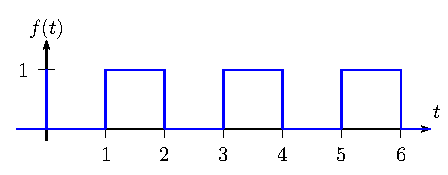
\includegraphics{cap_trans_int/pics/figura_24}\end{center}
\item[b)]~
\begin{center}

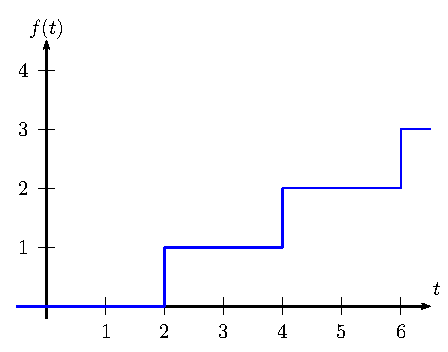
\includegraphics{cap_trans_int/pics/figura_25}\end{center}
\end{itemize}
\end{exer}
\begin{resp}
 \begin{itemize}
        \item[a)] $\displaystyle F(s)=\frac{e^{-s}}{s(1+e^{-s})}$
        \item[b)] $\displaystyle F(s)=\frac{e^{-2s}}{s(1-e^{-2s})}$ 
 \end{itemize}
\end{resp}

 \begin{exer}Use as propriedades de translação e a tabela de transformadas para calcular as transformadas inversa de Laplace da função $F(s)$:
 \begin{itemize}
  \item[a)] $\displaystyle F(s)=\frac{2s}{s^2+2s+5}$
    \item[b)] $\displaystyle F(s)=\frac{2s-2}{(s^2-2s+5)(s^2-2s+10)}$
  \item[c)] $\displaystyle F(s)=\frac{2e^{-4s}}{s^2-4}$
    \item[d)] $\displaystyle F(s)=2\frac{e^{-2s}}{(s-3)(s-1)}$
    \item[e)] $\displaystyle F(s)=\frac{2s}{s^2+2s+5}e^{-s}$
    \item[f)] $\displaystyle F(s)=\frac{2s-2}{(s^2-2s+5)(s^2-2s+10)}e^{-3s}$
 \end{itemize}
\end{exer}
\begin{resp}
\begin{itemize}
  \item[a)] $\displaystyle f(t)=\left(2\cos(2t)-\sen(2t)\right)e^{-t}$ 
      \item[b)] $\displaystyle f(t)=\frac{2e^{t}}{5}\left(\cos(2t)-\cos(3t)\right)$ 
        \item[c)] $\displaystyle f(t)=u(t-4)\senh(2(t-4))$ 
      \item[d)] $\displaystyle f(t)=u(t-2)\left(e^{3(t-2)}-e^{(t-2)}\right)$ 
        \item[e)] $\displaystyle f(t)=u(t-1)e^{-(t-1)}\left(2\cos(2(t-1))-\sen(2(t-1))\right)$ 
      \item[f)] $\displaystyle f(t)=2\frac{u(t-3)e^{t-3}}{5}\left(\cos(2(t-3))-\cos(3(t-3))\right)$ 
 \end{itemize}
\end{resp}
\begin{exer}Esboce o gráfico e calcule a transformada de Laplace das seguintes funções:
 \begin{itemize}
  \item[a)] $f(t)=tu(t-1)$
  \item[b)] $f(t)=t^2u(t-1)$
 \end{itemize}
\end{exer}
\begin{resp}
 \begin{itemize}
  \item[a)] $F(s)=\left(\frac{1}{s^2}+\frac{1}{s}\right)e^{-s}$
      \item[b)] $F(s)=\left(\frac{2}{s^3}+\frac{2}{s^2}+\frac{1}{s}\right)e^{-s}$
 \end{itemize}
\end{resp}
\begin{exer}
Mostre que:
\begin{itemize}
  \item[a)] $\displaystyle \mathcal{L}\{ \cosh (at) \sen (at) \} = \frac{a (s^2 + 2 a^2)}{s^4 + 4a^4}$
  \item[b)] $\displaystyle \mathcal{L} \{ \senh (at) \cos (at) \} = \frac{a (s^2 - 2 a^2)}{s^4 + 4a^4}$
  \item[c)] $\displaystyle \mathcal{L} \{ \senh (at) \sen (at) \} = \frac{2 a^2 s}{s^4 + 4a^4}$
\end{itemize}
 \noindent A partir destas, mostre que 
 \begin{equation}\mathcal{L}^{-1}\left\{ \frac{1}{s^4 + 4a^4}\right\} = \frac{1}{4a^3} \left[\cosh (at) \sen (at) - \senh (at) \cos(at)\right].   
 \end{equation}

\end{exer}
\begin{exer}
Encontre a transformada inversa das funções $F(s)$ abaixo:
\begin{itemize}
  \item[a)] $\displaystyle \frac{n\pi}{(s+2)^2 + n^2\pi^2}$
  \item[b)] $\displaystyle \frac{s}{(s+3)^2+1}$
  \item[c)] $\displaystyle \frac{6s-4}{s^2 - 4s +20}$
  \item[d)] $\displaystyle \frac{4s + 12}{s^2 + 8s + 16}$
\end{itemize}
\end{exer}
\begin{resp}
\begin{itemize}
\item[a)] $\displaystyle e^{-2t} \sen (n\pi t)$
  \item[b)] $\displaystyle e^{-3t} (\cos t - 3\sen  t)$
  \item[c)] $e^{2t} \big(6\cos (4t) + 2 \sen (4t)\big)$
  \item[d)] $\displaystyle 4e^{-4t} (1-t)$
\end{itemize}
  \end{resp}
  \begin{exer}
Encontre $g(t)$ e faça um esboço de seu gráfico, sendo $\mathcal{L}\{ g(t)\}$ igual a:
\begin{itemize}
  \item[a)] $\displaystyle \frac{2e^{-2s} - 2 e^{-4s}}{s}$
  \item[b)] $\displaystyle \frac{e^{-as}}{s^2}$
  \item[c)] $\displaystyle \frac{se^{-\pi s}}{s^2+4}$
  \item[d)] $\displaystyle \frac{e^{-\pi s}}{s^2 + 2s +2}$
  \item[e)] $\displaystyle \frac{e^{-s}+ e^{-2s} -3 e^{-3s} +6 e^{-6s}}{s^2}$
\end{itemize}
\end{exer}
\begin{resp}
\begin{itemize}
\item[a)] $\displaystyle 2 \big( u(t-2) - u(t-4) \big)$
  \item[b)] $\displaystyle (t-a)u(t-a)$
  \item[c)] $\displaystyle \cos\big(2(t-\pi)\big)u(t-\pi)$
  \item[d)] $\displaystyle e^{-(t-\pi)} \sen(t-\pi)u(t-\pi)$
  \item[e)] $\displaystyle (t-1)u(t-1) + (t-2)u(t-2) -3(t-3)u(t-3) + 6(t-6)u(t-6)$
\end{itemize}
\end{resp}
  
\section{A propriedade da transformada de Laplace da integral de uma função}
\begin{teo}{\label{prop_trans_int}}(Propriedade da transformada da integral) Se $F(s)$ é a transformada de Laplace de uma função contínua por partes $f(t)$, então $\int_0^tf(\tau)d\tau$ é a transformada inversa de $\frac{1}{s}F(s)$, isto é
\begin{equation}{\label{eq_trans_int}}
\mathcal{L}\left\{\int_0^tf(\tau)d\tau\right\} =\frac{1}{s}F(s),
\end{equation}
ou
\begin{equation}{\label{eq_trans_int_inv}}
\mathcal{L}^{-1} \left\{\frac{1}{s}F(s)\right\} =\int_0^tf(\tau)d\tau.
\end{equation} 
\end{teo}
\begin{proof}Seja $g(t)=\int_0^tf(\tau)d\tau$. Então $g'(t)=f(t)$. Aplicamos a propriedade da transformada da derivada \ref{prop_der} e temos:
\begin{equation}
\mathcal{L}\{g'(t)\}=s\mathcal{L}\{g(t)\}-g(0).
\end{equation}
Usando o fato que $g(0)=0$, temos
\begin{eqnarray*}
\mathcal{L}\left\{\int_0^tf(\tau)d\tau\right\}&=&\mathcal{L}\left\{g(t)\right\}\\
&=&\frac{1}{s}\mathcal{L}\{g'(t)\}\\
&=&\frac{1}{s}\mathcal{L}\{f(t)\}\\
&=&\frac{1}{s}F(s).
\end{eqnarray*}
\end{proof}
Essa propriedade será útil na aplicação de um circuito RC discutido na seção \ref{sec_circ}.
\subsection*{Exercícios}
\begin{exer}
Use a propriedade da transformada da integral para calcular $f(t)$ sabendo que $\mathcal{L}\{f \} $ é:
\begin{itemize}
  \item[a)] $\displaystyle \frac{5}{s^3 - 5s}$
  \item[b)] $\displaystyle \frac{10}{s^3 - \pi s^2}$
  \item[c)] $\displaystyle \frac{1}{s^4 + s^2}$
\end{itemize}
\end{exer}

\section{Aplicação: circuito RC a um pulso de amplitude $V_0$.}{\label{sec_circ}}
Considere o circuito Resistor/Capacitor representado na figura \ref{fig_circ} com uma tensão $V(t)$ aplicada do tipo pulso,
\begin{equation}
V(t)=V_0\left(u(t-a)-u(t-b)\right).
\end{equation}
ou seja, o circuito estava em repouso até $t=a$ e foi aplicada a tensão $V_0$ entre $t=a$ e $t=b$.
\begin{figure}[!ht]
\begin{center}

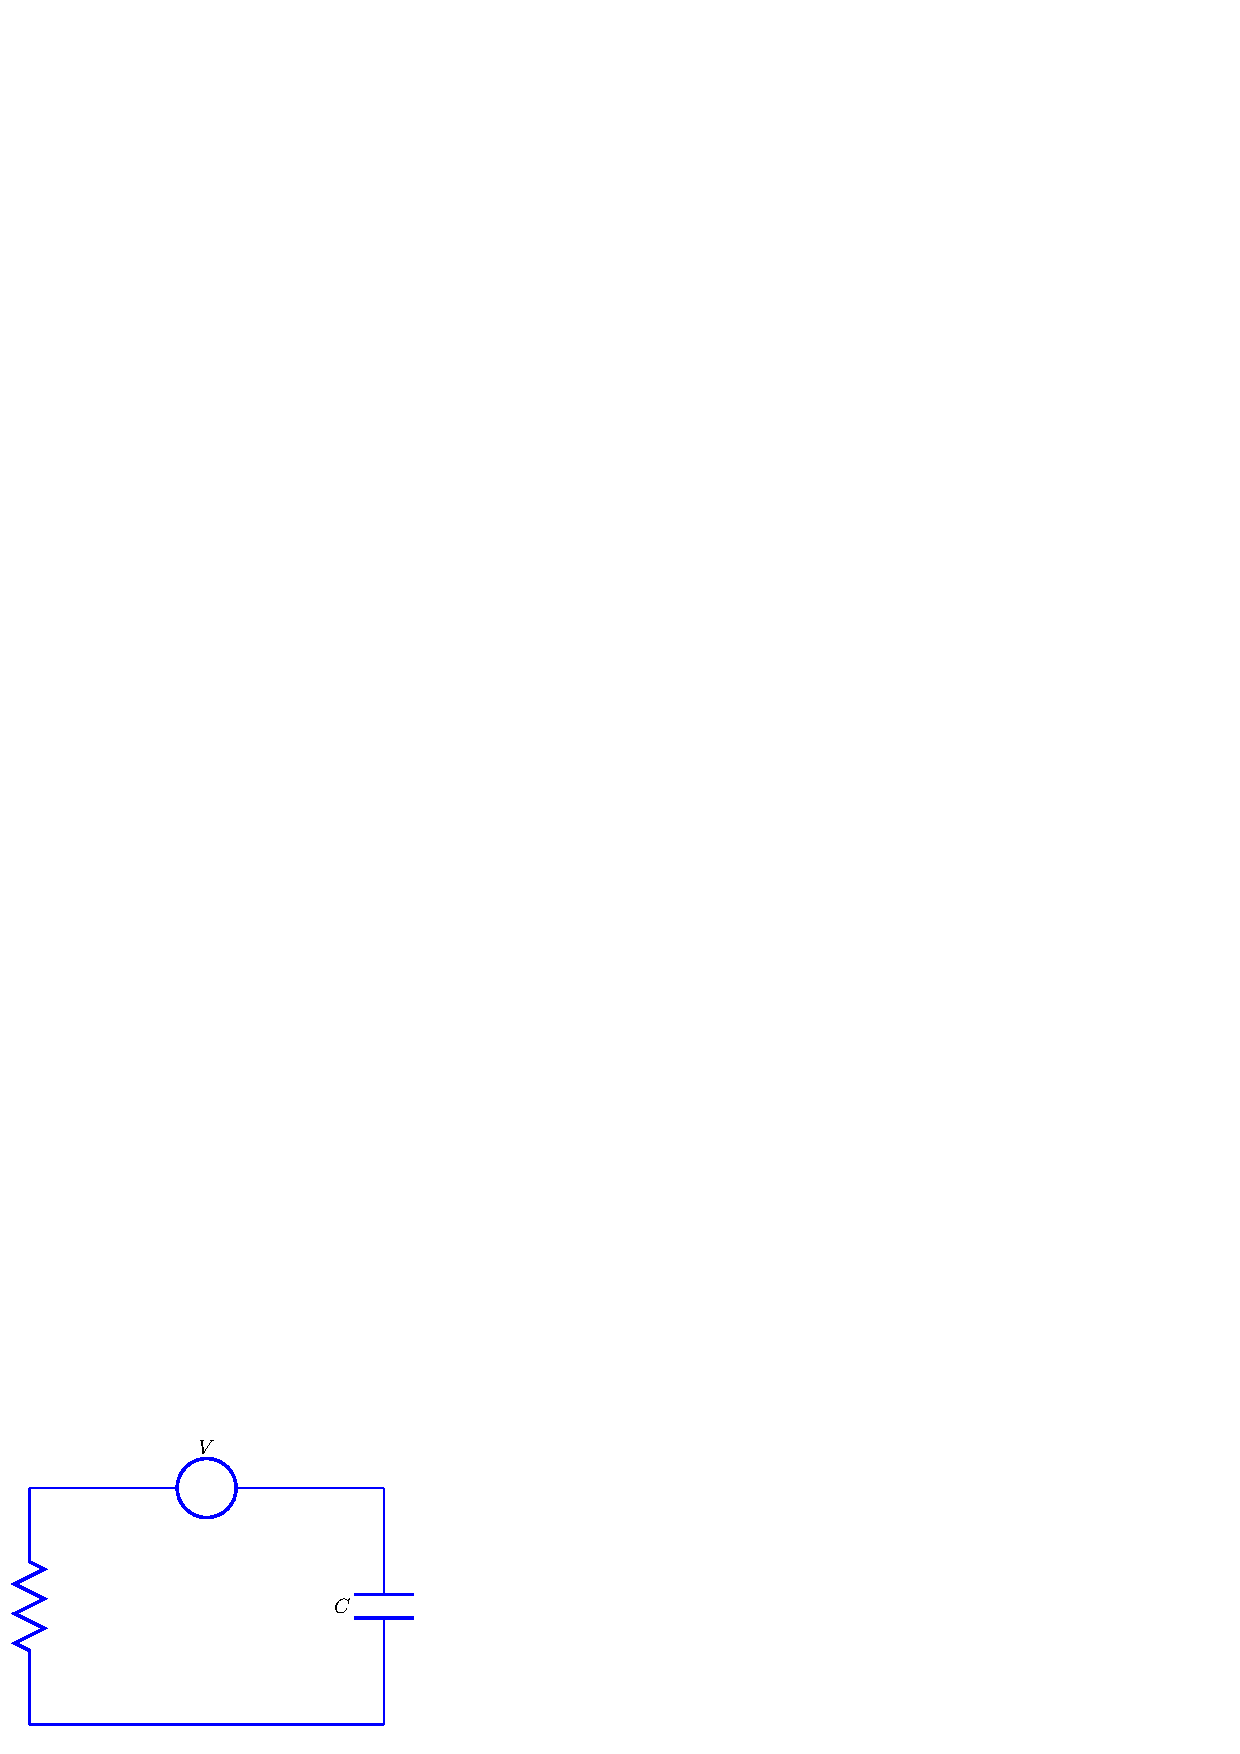
\includegraphics{cap_trans_int/pics/figura_10}\end{center}
\caption{\label{fig_circ}}
\end{figure}
O modelo para a corrente $i(t)$ obedece a lei de Kirchoff:
\begin{equation}{\label{modelo_corrente_0}}
 Ri(t)+\frac{1}{C}q(t)=V(t),
\end{equation}
onde $q(t)$ é a carga no capacitor, $\frac{1}{C}q(t)$ é a tensão no capacitor de capacitância $C$ e $Ri(t)$ é a tensão no resistor de resistência $R$. Usando o fato que $q(t)=\int_0^t i(\tau)d\tau$, obtemos uma equação integral para $i(t)$:
\begin{equation}
Ri(t)+\frac{1}{C}\int_0^t i(\tau)d\tau=V_0\left(u(t-a)-u(t-b)\right).
\end{equation}
Para resolver esse problema de valor incial, aplicamos a transformada de Laplace na equação acima e usamos a propriedade \ref{prop_trans_int}:
\begin{equation}
\mathcal{L}\left\{i(t)\right\}+\frac{1}{sRC}\mathcal{L}\left\{i(t)\right\}=\frac{V_0}{Rs}\left(e^{-as}-e^{-bs}\right),
\end{equation}
ou seja, obtemos a seguinte equação subsidiária:
\begin{equation}
sI(s)+\frac{1}{RC}I(s)=\frac{V_0}{R}\left(e^{-as}-e^{-bs}\right),
\end{equation}
onde $I(s)=\mathcal{L}\left\{i(t)\right\}$. Logo,
\begin{equation}
I(s)=\frac{V_0 C}{RCs+1}\left(e^{-as}-e^{-bs}\right)=\frac{V_0}{R}\frac{1}{s+\frac{1}{RC}}\left(e^{-as}-e^{-bs}\right).
\end{equation}
O item 7 da tabela de transformadas \ref{tab_trans_Lap_1} nos dá $\mathcal{L}^{-1}\left\{\frac{1}{s-d}\right\}=e^{dt}$. Tome $d=-\frac{1}{RC}$ e obtemos
\begin{equation}
\mathcal{L}^{-1}\left\{\frac{1}{s+\frac{1}{RC}}\right\}=e^{-\frac{t}{RC}}.
\end{equation}
Agora, usamos a propriedade \ref{prop_trans_t} do deslocamento no eixo $t$ para calcular a função corrente:
\begin{eqnarray*}
i(t)&=&\mathcal{L}^{-1}\left\{\frac{V_0}{R}\frac{1}{s+\frac{1}{RC}}\left(e^{-as}-e^{-bs}\right)\right\}\\
&=&\frac{V_0}{R}\left[\mathcal{L}^{-1}\left\{\frac{1}{s+\frac{1}{RC}}e^{-as}\right\}-\mathcal{L}^{-1}\left\{\frac{1}{s+\frac{1}{RC}}e^{-bs}\right\}\right]\\
&=&\frac{V_0}{R}\left[u(t-a)e^{-\frac{(t-a)}{RC}}-u(t-b)e^{-\frac{(t-b)}{RC}}\right]\\
&=&\frac{V_0}{R}\left[u(t-a)e^{\frac{a}{RC}}-u(t-b)e^{\frac{b}{RC}}\right]e^{-\frac{t}{RC}}.
\end{eqnarray*}
Olhando numa notação de função definida por partes, podemos escrecer
\begin{equation}
i(t)=\left\{\begin{array}{ll}0,&t<a  \\A e^{-\frac{t}{RC}}, &a<t<b, \\ \left(A-B\right)e^{-\frac{t}{RC}}, &t>b, \end{array}\right.
\end{equation}
onde
\begin{equation}
A=\frac{V_0}{R}e^{\frac{a}{RC}}\qquad\hbox{e}\qquad B=\frac{V_0}{R}e^{\frac{b}{RC}}.
\end{equation}
Observe que $A>0$, $B>0$ e $A<B$, ou seja, para $t>b$ a corrente é negativa e se aproxima exponencialmente de zero. Essa é a chamada corrente de descarga. A figura \ref{fig_circ_1} apresenta um gráfico da corrente quando $a=0.5$, $b=2$, $R=1\Omega$, $C=1\ \!$F e $V_0=3V$.

Para obter a carga no capacitor usamos $q(t)=\int_0^t i(\tau)d\tau$ e obtemos a seguinte expressão:
\begin{equation}\label{eq:sol_carga}
q(t)=\left\{\begin{array}{ll}0,&t<a  \\ CV_0\left(1-e^{-\frac{t-a}{CR}}\right), &a<t<b, \\ CV_0\left(e^{-\frac{t-b}{CR}}-e^{-\frac{t-a}{CR}} \right), &t>b, \end{array}\right.
\end{equation}

A figura \ref{fig_circ_10} apresenta um gráfico da carga quando $a=0.5$, $b=2$, $R=1\Omega$, $C=1\ \!$F e $V_0=3V$. Observe a consitência com o gráfico da figura \ref{fig_circ_1}.


\begin{figure}[!ht]
\begin{center}

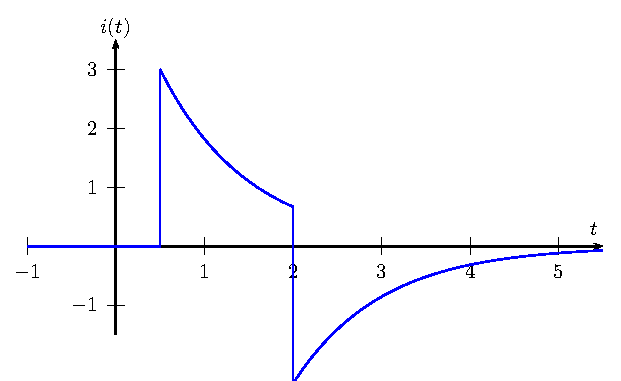
\includegraphics{cap_trans_int/pics/figura_11}\end{center}
\caption{\label{fig_circ_1}}
\end{figure}
\begin{figure}[!ht]
\begin{center}

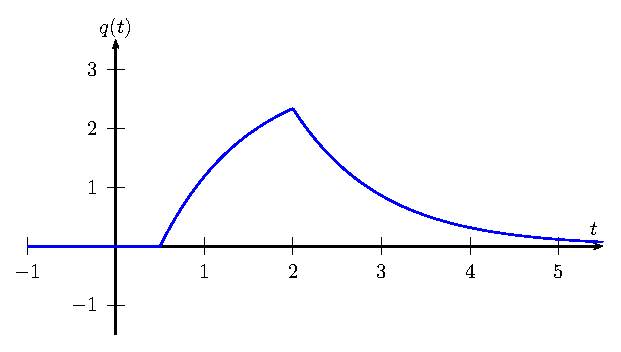
\includegraphics{cap_trans_int/pics/figura_12}\end{center}
\caption{\label{fig_circ_10}}
\end{figure}




\subsection*{Exercícios}
\begin{exer}
Use as equações \eqref{modelo_corrente_0} $i(t)=\frac{dq(t)}{dt}$ para obter uma equação diferencial ordinária para a carga $q(t)$. Depois resolva-o usando transformada de Laplace e obtenha a solução \eqref{eq:sol_carga}.
\end{exer}
\begin{resp}
Voltamos a equação (\ref{modelo_corrente_0}) e usamos $i(t)=\frac{dq(t)}{dt}$
\begin{equation}
 Rq'(t)+\frac{1}{C}q(t)=V_0\left(u(t-a)-u(t-b)\right).
\end{equation}
Obtemos a equação subsidiária aplicando a transformada de Laplace:
\begin{equation*}
  R\left(sQ(s)-q(0)\right)+\frac{1}{C}Q(s)=\frac{V_0}{s}\left(e^{-as}-e^{-bs}\right).
\end{equation*}
onde $Q(s)=\mathcal{L}\{q(t)\}$. Como o fenômeno estava em repouso no início, $q(0)=0$. A solução da equação subsidiária é
\begin{equation}
Q(s)=\frac{C}{RCs+1}\frac{V_0}{s}\left(e^{-as}-e^{-bs}\right)=\frac{V_0}{R}\frac{1}{s\left(s+\frac{1}{CR}\right)}\left(e^{-as}-e^{-bs}\right).
\end{equation}
O item 11 da tabela \ref{tab_trans_Lap_1} nos dá 
\begin{equation}
\mathcal{L}^{-1}\left\{\frac{1}{(s-d_1)(s-d_2)}\right\}=\frac{1}{d_1-d_2}\left(e^{d_1t}-e^{d_2t}\right).
\end{equation}
Colocamos $d_1=0$, $d_2=-\frac{1}{CR}$ 
\begin{equation}
\mathcal{L}^{-1}\left\{\frac{1}{s\left(s+\frac{1}{CR}\right)}\right\}=CR\left(1-e^{-\frac{t}{CR}}\right).
\end{equation}
Agora usamos a propriedade \ref{prop_trans_t} da translação no eixo $t$ e obtemos:
\begin{equation}
q(t)=CV_0\left(u(t-a)\left(1-e^{-\frac{t-a}{CR}}\right)-u(t-b)\left(1-e^{-\frac{t-b}{CR}}\right) \right),
\end{equation}
que coincide com a solução dada na equação \eqref{eq:sol_carga}.
\end{resp}









